\section{Development method}
The task given to us was open because we had few restrictions, and it was up to our group to decide which technologies to use. This meant that work methodology had to focus more on flexibility rather than planning. We therefore chose to use an agile work method. Agile work method focuses on continuous planning throughout the process, and having frequent communication with the client, in our case Accenture. We had meetings with our external supervisors from Accenture once every second week which meant the agile work was a good fit for our project. 

We chose to use inspiration from two light frameworks, kanban and scrum. Scrum is an agile,  light framework which helps people and teams work together. Scrum describes a set of meetings, roles and tools.

\begin{figure}[h!]
	\centering
	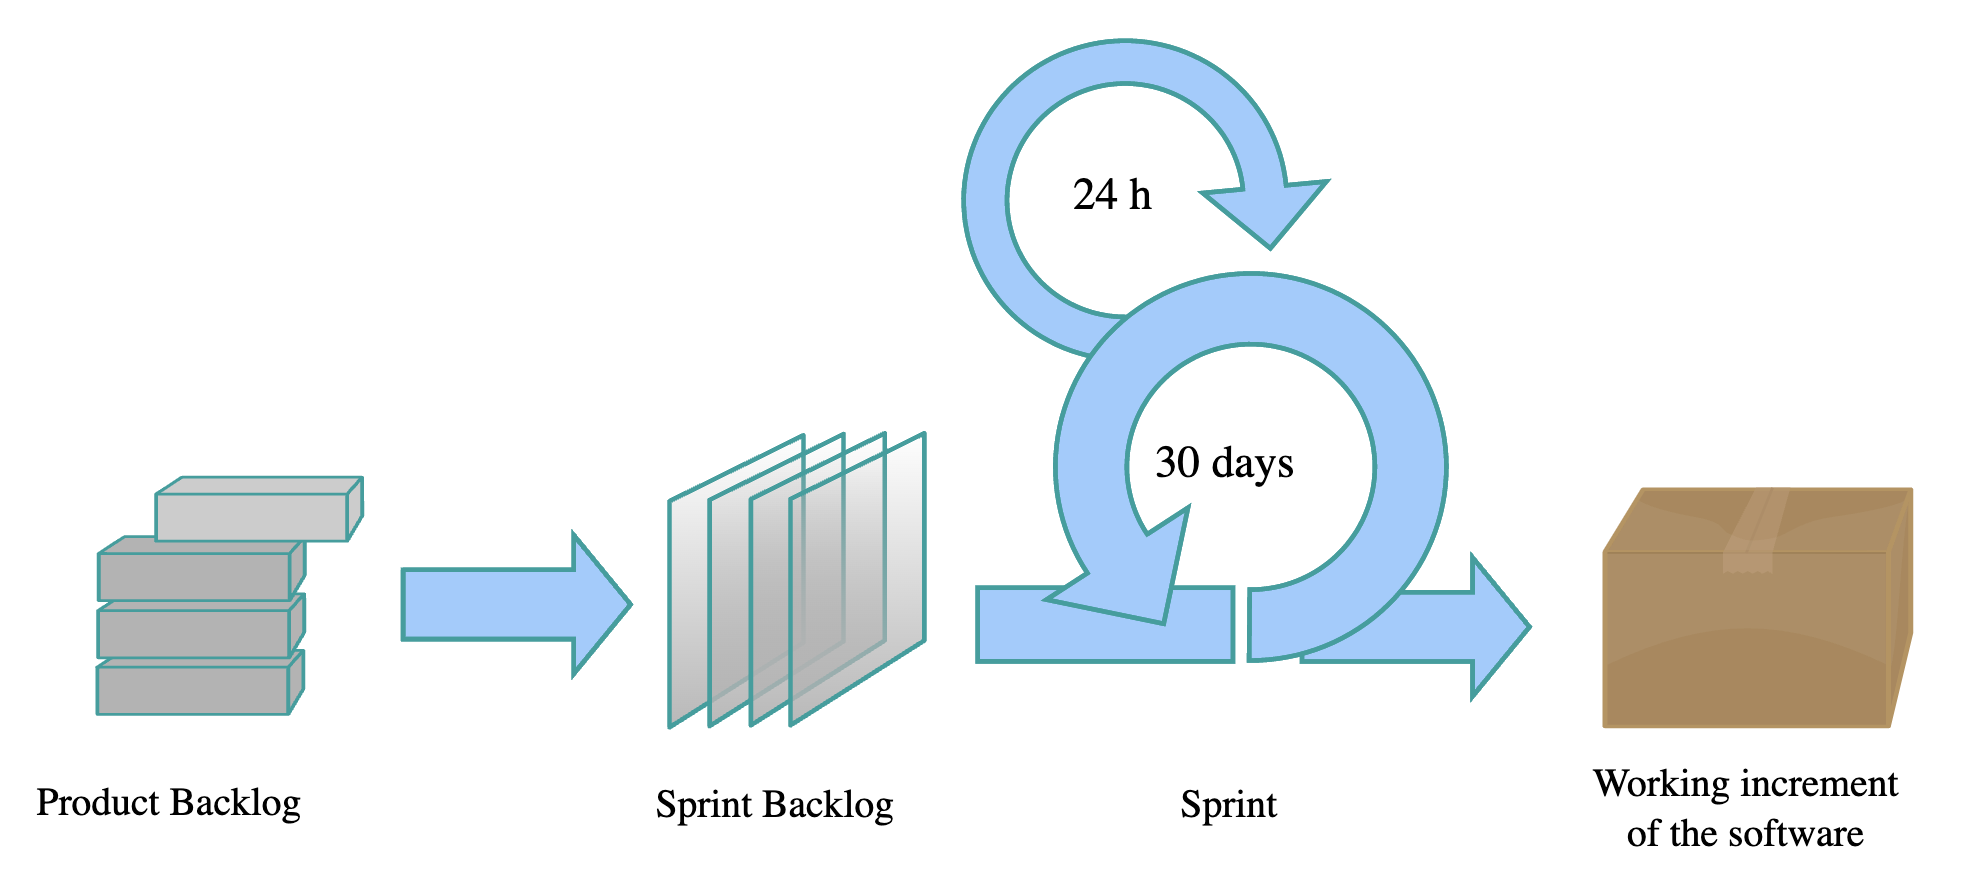
\includegraphics[width=1\linewidth]{figures/scrum_process}
	\caption[scrum process]{Illustration of a generic scrum process.}
	\label{fig:scrumprocess}
\end{figure}


A sprint is an essential part in using the Scrum framework. Sprints are a fixed time length, often between one and four weeks. In this specified time length the teams do tasks assigned from the sprint backlog . Each sprint starts with a sprint planning and ends with a sprint retro perspective. For our project we found it most viable to plan in increments of two weeks. We chose two weeks increments because we felt it was an even balance between work and planning. As mentioned we also had meetings with our client Accenture every 2 weeks which fitted well with the time increment.  

Our group also made use of the meetings in the Scrum framework. The meetings are sprint planning, sprint retroperspective and daily standups. Sprint planning is a meeting or event which starts before a sprint. At the sprint planning the teams agree on a goal for the sprint, and the tasks from the backlog that should be worked on that contribute to the goal. Example of report from a sprint planning meeting is attached. The backlog is a list of functionality the product should contain. In addition we wrote down the tasks for the specific sprints in a digital document. These tasks were to be finished by the next sprint. Here is our sprint planning documents that shows our goals for each sprint:

(Legge til figur av sprint planning documentet vårt)

After a sprint we would have a sprint retro perspective where we would discuss what went well in that sprint, and what could have been done better. This helped us reflect over the prior week and adjust accordingly, if necessary. We would also discuss if the task asigned in the sprint meetings were finnished or needed more work. This helped us figure out if we were on track with our initial plan. 
 
In addition to the weekly meetings we also had daily standups. Daily standups is a short meeting, usually around five minutes, where each person answers three questions. What did you do last time? What are you doing today? Are there any challenges? We implemented daily standups because it helped our team get on the same page, and it made it easier to plan what each of us had to do that specific day.

Scrum often consists of a team with different roles. As a team of three where we did not feel the necessity to have specified roles, because we usually worked together on our project. However we alternated on being the scrum master. The scrum master’s responsibility is to keep track of the backlog and lead the sprint planning meetings.

Our implementation of Kanban was to use a Kanban board as the backlog. A Kanban board is used to visualize where a task is in the work process. Here is an example from our project:

\begin{figure}[h!]
	\centering
	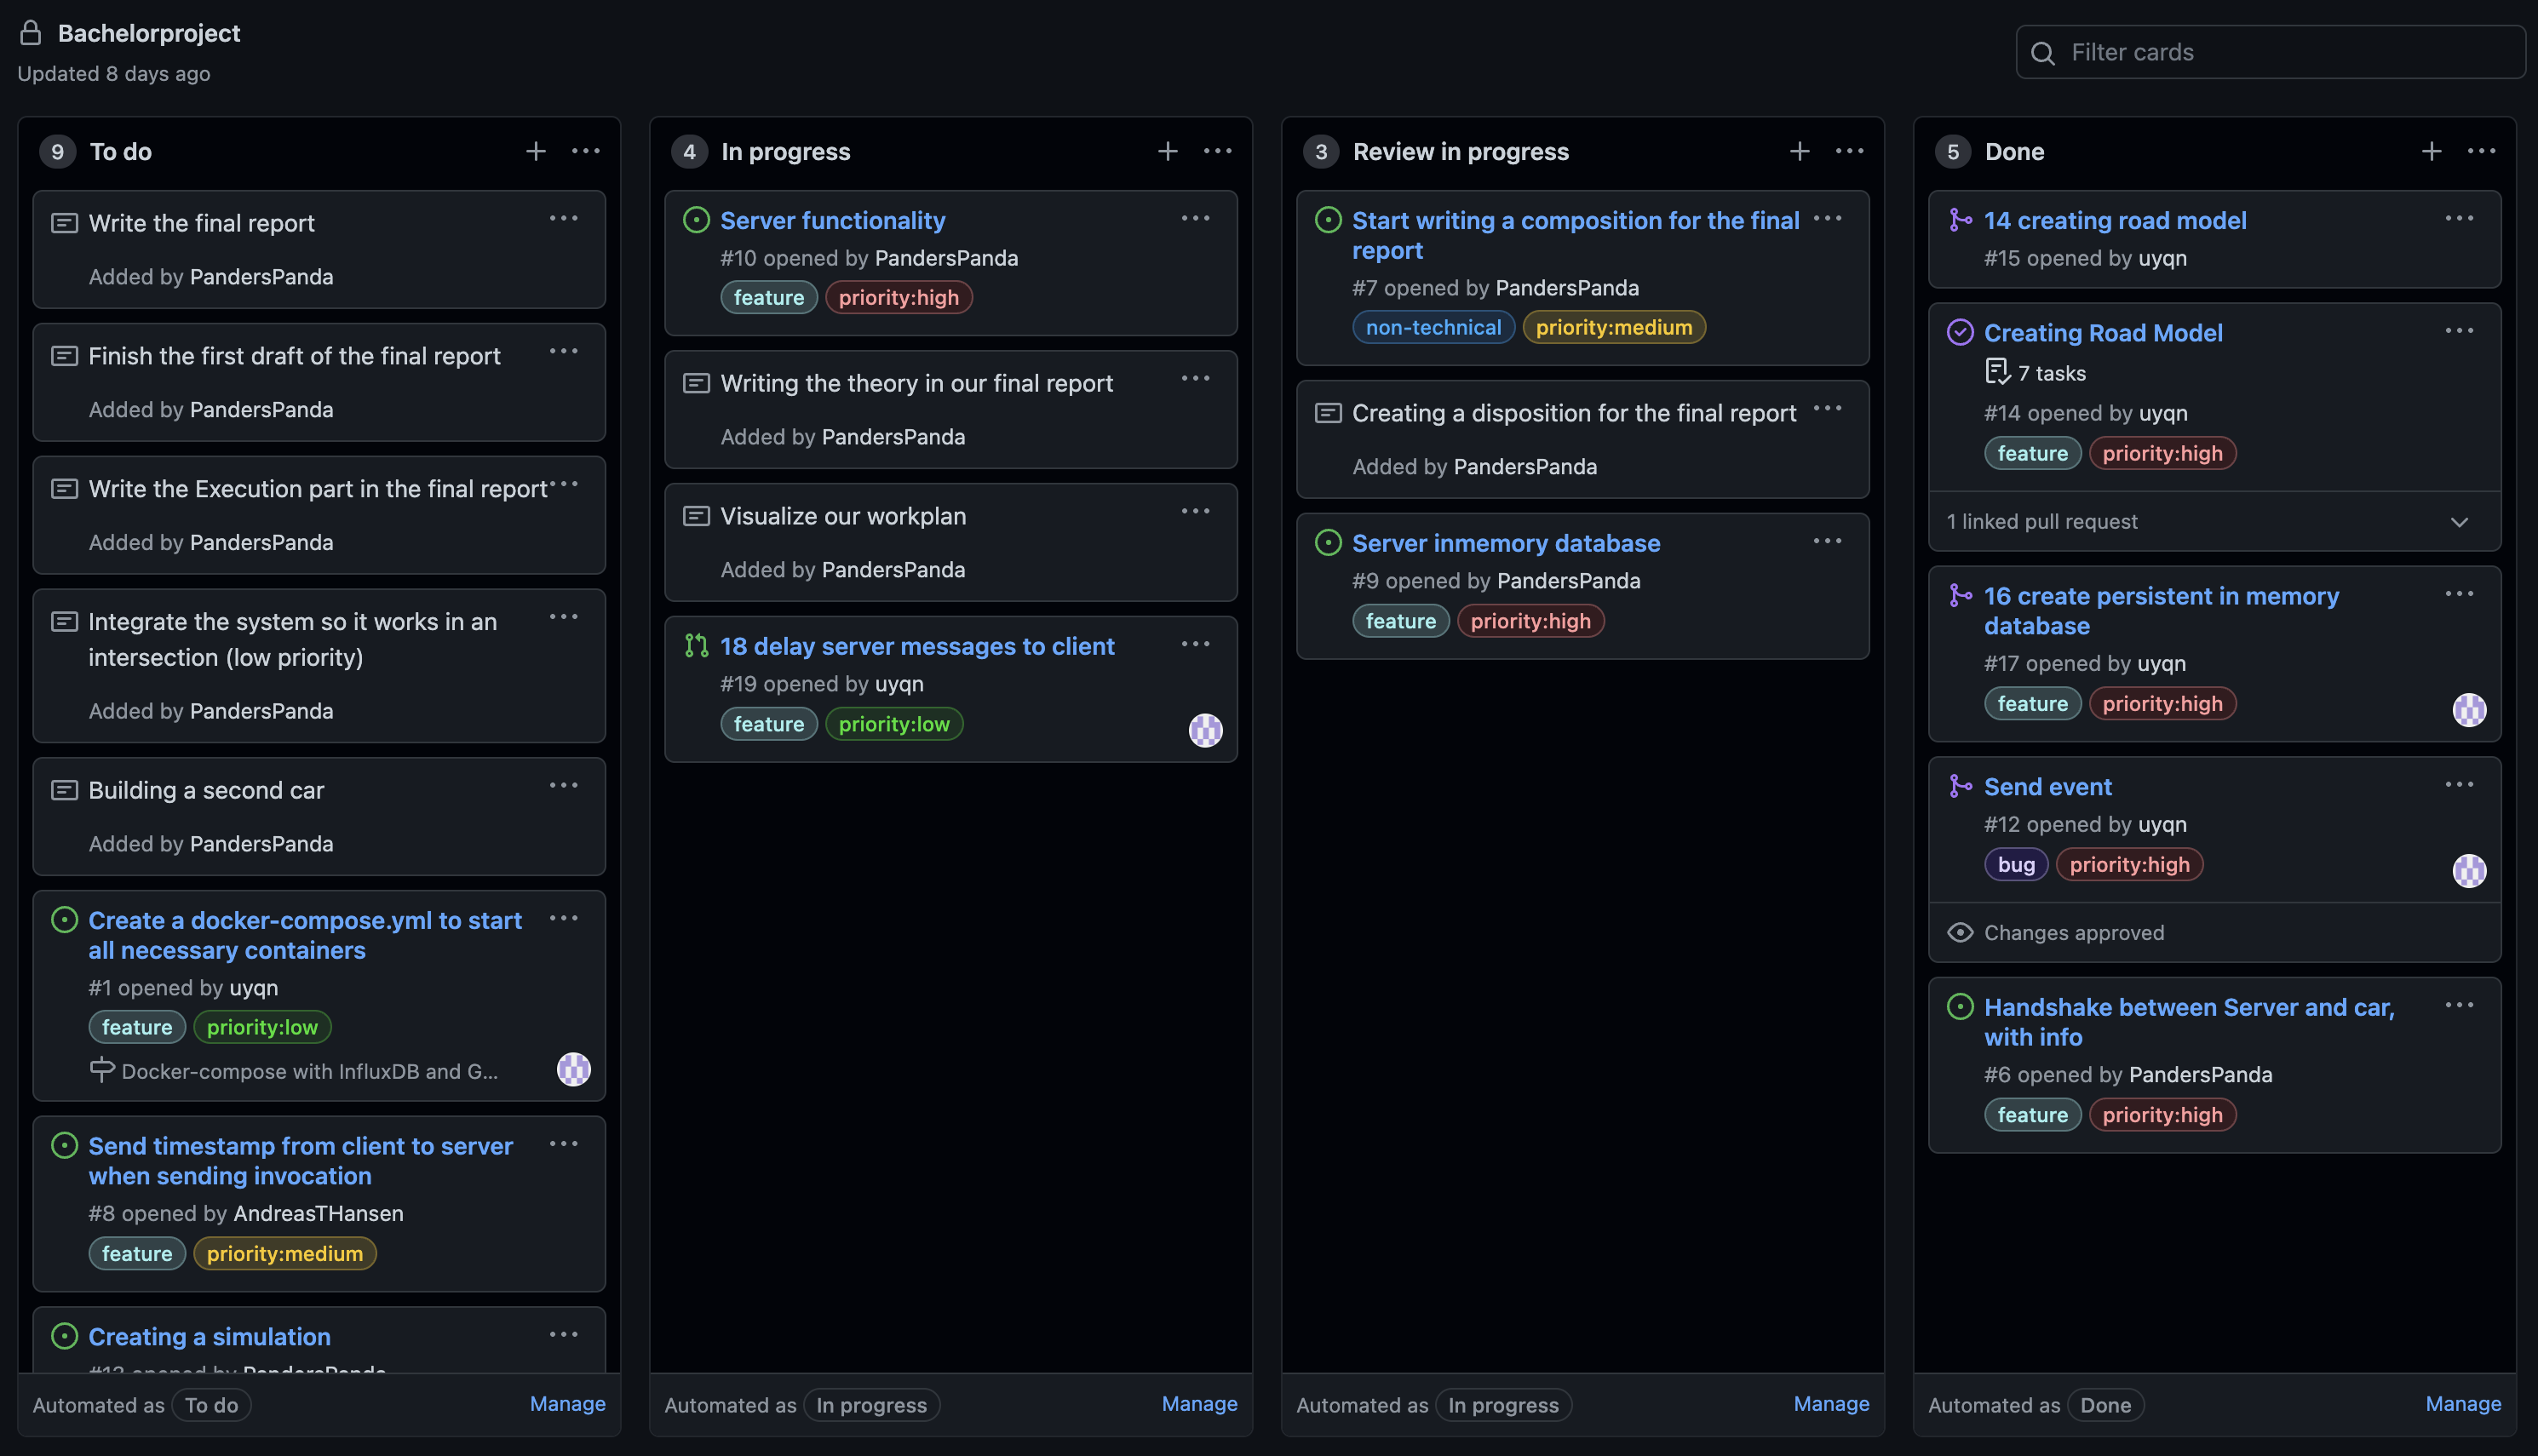
\includegraphics[width=1\linewidth]{figures/kanban_screenshot}
	\caption[kanban screenshot]{Extract of our kanban from Github.}
	\label{fig:kanbanscreenshot}
\end{figure}

We have four columns that represent which phase a task is in. The backlog is the tasks in the to-do column. When we are working on a task we drag it over to the In progress column. After a task is finished it goes to the “Review in progress”, where we test it. If the testing is a success it gets dragged over to the “Done column”. The Kanban board was a great tool to see which tasks to choose for our sprints, and also keep track of where the tasks were in their process.

However, we did not use the Canban board thoughout the whole prosess. This is because the backlog was changing a lot, and therefore the canban board needed many modifications to be up to date. In addition, we were able to keep track of the tasks by having frequent meetings.We figured out that it was more beneficial to focus on one framwork, which in our case was scrum. 